\chapter{Validation (part 2): formal schemes}\label{ch-10}

This second part formalises the correct use of cross-validation for
model selection and/or risk estimation, with precise notation (adapted
from S. Bengio's slides). The concepts are simple, but rigorous notation
avoids ambiguity. It is not a cookbook: it serves to
\textbf{rationalise} and systematically understand a rigorous approach,
so as to then be reasonable. The time needed to run the experiments
depends mainly on the validation choices: one must avoid both an overly
coarse evaluation and an endless evaluation process. When in doubt,
these schemes are in any case better than imagination.

We talk about selection among hyperparameter configurations (denoted
by \(\theta\)), but the same schemes apply to choosing among
\textbf{different models} (\(\theta\) can also represent the type of
model).

\begin{boxtip}{Keep the counterexample in mind}

From part 1: (1) error estimates on TR and/or VL are \textbf{not} good
estimates of the risk; (2) using the whole dataset for feature or model
selection \textbf{compromises} the estimate. In the schemes that follow
we see exactly where these errors would be made.

\end{boxtip}

\section{Notation}\label{notazione}

\textbf{Data}: \(Z_1, \dots, Z_l\) is a random sample from an unknown
distribution \(p(z)\), with all \(Z_i\) \textbf{independent and
identically distributed} (i.i.d.). \(D_r = \{z_1, \dots, z_r\}\) is a
particular instance with \(r\) elements.

\textbf{Task}: classification,
\(Z = (X, Y) \in \mathbb{R}^n \times \{-1, +1\}\); regression,
\(Z = (X, Y) \in \mathbb{R}^n \times \mathbb{R}\).

\textbf{Loss} (``inner''): classification \(L((x,y), h) = 0\) if
\(h(x) = y\), \(1\) otherwise; regression
\(L((x,y), h) = (h(x) - y)^2\).

\textbf{Goal}: minimise the \textbf{expected risk} (true error) over
\(H\): \[
R(h) = \mathbb{E}_Z[L(z, h)] = \int_Z L(z, h)\,p(z)\,dz, \qquad h^* = \arg\min_{h \in H} R(h).
\] The problem: \(p(z)\) is unknown and we do not have access to all
the \(L(z,h)\).

\textbf{Empirical risk} on a finite set \(D_r\): \[
R_{emp}(h, D_r) = \frac{1}{r}\sum_{i=1}^{r} L(z_i, h).
\]

\begin{boxwarning}{General use of \(R_{emp}\)}

Here \(R_{emp}\) is meant in a general sense, as a \textbf{surrogate of
\(R\)} on a finite set of data, used for training, model selection or
assessment depending on the partition. Not to be confused with the SLT
\(R_{emp}\), which is specifically the training error: in this notation
it is \(R_{emp}(h, D_{TR})\).

\end{boxwarning}

\section{Methodology: identifying the
goal}\label{metodologia-identificare-lobiettivo}

\begin{enumerate}
\def\labelenumi{\arabic{enumi}.}
\tightlist
\item
  Provide the \textbf{best model} obtainable from a dataset? →
  \textbf{model selection} is needed.
\item
  Provide the \textbf{expected performance} of a model obtained by
  empirical risk minimisation? → \textbf{model assessment} (risk
  estimation) is needed.
\item
  Provide \textbf{both}? → both are needed.
\end{enumerate}

The original dataset \(D_l\) will be used for these different purposes.

\section{Model selection}\label{model-selection}

\subsection{Hold-out}\label{hold-out}

\begin{boxabstract}{Model selection with hold-out}

\begin{itemize}
\tightlist
\item
  Choose a hypothesis space with hyperparameter \(\theta\).
\item
  Split \(D_l\) into \(D_{TR} = \{z_1, \dots, z_{tr}\}\) and
  \(D_{VL} = \{z_{tr+1}, \dots, z_{tr+vl}\}\), with \(tr + vl = l\).
\item
  For each value \(\theta_m\) {[}\textbf{grid search}{]}:

  \begin{itemize}
  \tightlist
  \item
    \(h^*_{\theta_m}(D_{TR}) = \arg\min_{h \in H_{\theta_m}} R_{emp}(h, D_{TR})\)
    {[}\textbf{training}{]};
  \item
    estimate \(R(h^*_{\theta_m})\) with
    \(R_{emp}(h^*_{\theta_m}, D_{VL}) = \frac{1}{vl}\sum_{z_i \in D_{VL}} L(z_i, h^*_{\theta_m}(D_{TR}))\).
  \end{itemize}
\item
  Choose \(\theta^*_m = \arg\min_{\theta_m} R(h^*_{\theta_m})\)
  {[}best result on VL{]}.
\item
  Return
  \(h^*(D_l) = \arg\min_{h \in H_{\theta^*_m}} R_{emp}(h, D_l)\)
  {[}\textbf{retraining} on all \(l\) data{]}.
\end{itemize}

\end{boxabstract}

The estimate of \(R\) on VL serves \textbf{only} for model selection
and \textbf{is not returned} as a risk estimate: returning it would be
exactly error (1) of the counterexample.

\subsection{K-fold cross-validation}\label{k-fold-cross-validation}

\begin{boxabstract}{Model selection with K-fold CV}

\begin{itemize}
\tightlist
\item
  Choose a hypothesis space with hyperparameter \(\theta\).
\item
  Split \(D_l\) into \(K\) distinct, equal parts \(D_1, \dots, D_K\);
  let \(\bar D_k\) be the complement of \(D_k\).
\item
  For each value \(\theta_m\) {[}\textbf{grid search}{]}:

  \begin{itemize}
  \tightlist
  \item
    for each part \(D_k\) {[}\textbf{loop over folds}{]}:

    \begin{itemize}
    \tightlist
    \item
      \(h^*_{\theta_m}(\bar D_k) = \arg\min_{h \in H_{\theta_m}} R_{emp}(h, \bar D_k)\)
      {[}training{]};
    \item
      estimate \(R(h^*_{\theta_m}(\bar D_k))\) with
      \(R_{emp}(h^*_{\theta_m}(\bar D_k), D_k) = \frac{1}{|D_k|}\sum_{z_i \in D_k} L(z_i, h^*_{\theta_m}(\bar D_k))\);
    \end{itemize}
  \item
    estimate \(R(h^*_{\theta_m}(D_l))\) with the mean
    \(\frac{1}{K}\sum_k R(h^*_{\theta_m}(\bar D_k))\).
  \end{itemize}
\item
  Choose \(\theta^*_m = \arg\min_{\theta_m} R(h^*_{\theta_m}(D_l))\)
  {[}best over all CVs{]}.
\item
  Return
  \(h^*(D_l) = \arg\min_{h \in H_{\theta^*_m}} R_{emp}(h, D_l)\)
  {[}retraining{]}.
\end{itemize}

\end{boxabstract}

\begin{figure}[htbp]
\centering
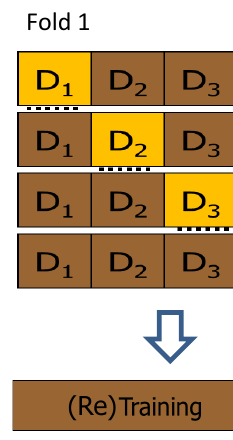
\includegraphics[width=0.31\linewidth,height=0.42\textheight,keepaspectratio]{images/10-val2_kfold-selezione.png}
\caption{K-fold CV for model selection, followed by retraining.}
\end{figure}

\begin{boxwarning}{Beware of the order}

Each iteration \textbf{starts from scratch}, with training and
estimation local to the split. If for example a model trained in split
1 were used to evaluate split 2, a part (\(D_2\)) that had been used for
training in split 1 would be used as validation for split 2.

\end{boxwarning}

\section{Risk estimation (model
assessment)}\label{stima-del-rischio-model-assessment}

\subsection{Hold-out}\label{hold-out-1}

\begin{boxabstract}{Model assessment with hold-out}

\begin{itemize}
\tightlist
\item
  Split \(D_l\) into \(D_{TR}\) and \(D_{TS}\), with \(tr + ts = l\).
  \textbf{The test set must be separated NOW} (not later): otherwise
  error (2) of the counterexample is made.
\item
  \(h^*(D_{TR}) = \arg\min_{h \in H} R_{emp}(h, D_{TR})\) {[}training;
  it may include an internal model selection on \(D_{TR}\){]}.
\item
  Estimate \(R(h^*(D_{TR}))\) with
  \(R_{emp}(h^*(D_{TR}), D_{TS}) = \frac{1}{ts}\sum_{z_i \in D_{TS}} L(z_i, h^*(D_{TR}))\)
  {[}\textbf{test error}{]}.
\end{itemize}

\end{boxabstract}

\subsection{K-fold cross-validation}\label{k-fold-cross-validation-1}

\begin{boxabstract}{Model assessment with K-fold CV}

\begin{itemize}
\tightlist
\item
  Split \(D_l\) into \(K\) distinct, equal parts.
\item
  For each part \(D_k\) {[}loop over folds{]}:

  \begin{itemize}
  \tightlist
  \item
    \(h^*(\bar D_k) = \arg\min_{h \in H} R_{emp}(h, \bar D_k)\)
    {[}training; it may include a model selection{]};
  \item
    estimate \(R(h^*(\bar D_k))\) with \(R_{emp}(h^*(\bar D_k), D_k)\)
    {[}test error of each iteration{]}.
  \end{itemize}
\item
  Estimate \(R(h^*(D_l))\) with the mean
  \(\frac{1}{K}\sum_k R(h^*(\bar D_k))\).
\end{itemize}

\end{boxabstract}

With \(K = l\) we have \textbf{leave-one-out CV}. The principles are
not violated: test results are never used for training or selection,
in any iteration.

\section{Combining model selection and model
assessment}\label{combinare-model-selection-e-model-assessment}

When both the best model and its expected risk are wanted, the methods
must be combined. For example:

\begin{itemize}
\tightlist
\item
  \textbf{hold-out} with training--validation--test (three separate
  sets are needed);
\item
  \textbf{K-fold CV + test}: cross-validation on the training set, then
  test on a separate set;
\item
  \textbf{external K-fold CV for the test}, with internal hold-out for
  model selection;
\item
  \textbf{double (nested) cross-validation}: for each external fold, a
  nested cross-validation on the other \(K-1\).
\end{itemize}

Other aspects: take into account the \textbf{different trials}
(different initialisations of a network) when computing the means on
TR, VL, TS. More generally: compare the results with other methods,
use \textbf{statistical tests} to check their significance, verify the
model on several datasets.

\subsection{Hold-out
training--validation--test}\label{hold-out-trainingvalidationtest}

\begin{boxabstract}{TR--VL--TS scheme}

\begin{itemize}
\tightlist
\item
  Split \(D_l\) into \(D_{TR}\), \(D_{VL}\), \(D_{TS}\).
\item
  For each \(\theta_m\): train \(h^*_{\theta_m}(D_{TR})\) and compute
  \(R_{emp}(h^*_{\theta_m}(D_{TR}), D_{VL})\).
\item
  Choose \(\theta^*_m\) with the best result on VL.
\item
  Retrain \(h^*(D_{TR} \cup D_{VL})\) with \(\theta^*_m\).
\item
  Estimate \(R\) with
  \(\frac{1}{ts}\sum_{z_i \in D_{TS}} L(z_i, h^*(D_{TR} \cup D_{VL}))\).
\end{itemize}

\end{boxabstract}

Retraining can use part of the data as VL for early stopping.

\begin{boxquestion}{Can one retrain again on the whole \(D_l\)?}

The final retraining on all the data (TR+VL+TS) \textbf{does not use}
the test results for any choice: the final model will in general have
performance equal to or better than the estimate (more data), which
remains valid as a (slightly pessimistic) estimate of the risk of the
procedure. What matters is that the test has not influenced any
decision.

\end{boxquestion}

\subsection{K-fold CV for selection + hold-out for the
test}\label{k-fold-cv-per-la-selezione-hold-out-per-il-test}

\begin{boxabstract}{CV + test scheme}

\begin{itemize}
\tightlist
\item
  Split \(D_l\) into \(D_{TR}\) (the \emph{design set}) and \(D_{TS}\).
\item
  For each \(\theta_m\): estimate \(R(h^*_{\theta_m}(D_{TR}))\) with a
  K-fold CV on \(D_{TR}\) (mean validation error over the folds).
\item
  Choose \(\theta^*_m\) with the best estimate.
\item
  Retrain \(h^*(D_{TR})\).
\item
  Estimate \(R\) with the error on \(D_{TS}\).
\end{itemize}

\end{boxabstract}

\subsection{K-fold CV for the test with internal hold-out for
selection}\label{k-fold-cv-per-il-test-con-hold-out-interno-per-la-selezione}

In each row of the external K-fold, one fold acts as test and the rest
is split (arbitrarily and with shuffling) into TR and VL for model
selection. The description as a meta-algorithm is left as an exercise.

\begin{figure}[htbp]
\centering
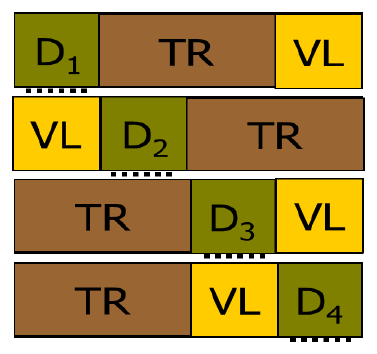
\includegraphics[width=0.31\linewidth,height=0.42\textheight,keepaspectratio]{images/10-val2_kfold-holdout.png}
\caption{External K-fold CV for the test, with internal TR/VL hold-out
for model selection (retraining is not shown).}
\end{figure}

\begin{boxnote}{No single model}

This process \textbf{does not provide a final model}: it only gives an
estimate of the risk of the \textbf{class} of models considered,
because potentially each row selects a different model.

\end{boxnote}

\subsection{Double (nested) K-fold CV}\label{double-nested-k-fold-cv}

\begin{boxabstract}{Double K-fold CV}

\begin{itemize}
\tightlist
\item
  Split \(D_l\) into \(K\) distinct, equal parts.
\item
  For each part \(D_k\) {[}\textbf{outer loop}{]}:

  \begin{itemize}
  \tightlist
  \item
    choose \(h^*(\bar D_k)\) with an \textbf{internal K-fold CV} on
    \(\bar D_k\) (with \(K'\) possibly different from \(K\))
    {[}\textbf{inner loop}{]};
  \item
    estimate \(R(h^*(\bar D_k))\) with \(R_{emp}(h^*(\bar D_k), D_k)\)
    {[}test error for each outer split{]}.
  \end{itemize}
\item
  Estimate \(R(h^*(D_l))\) with the mean over the test folds.
\end{itemize}

\end{boxabstract}

\begin{figure}[htbp]
\centering
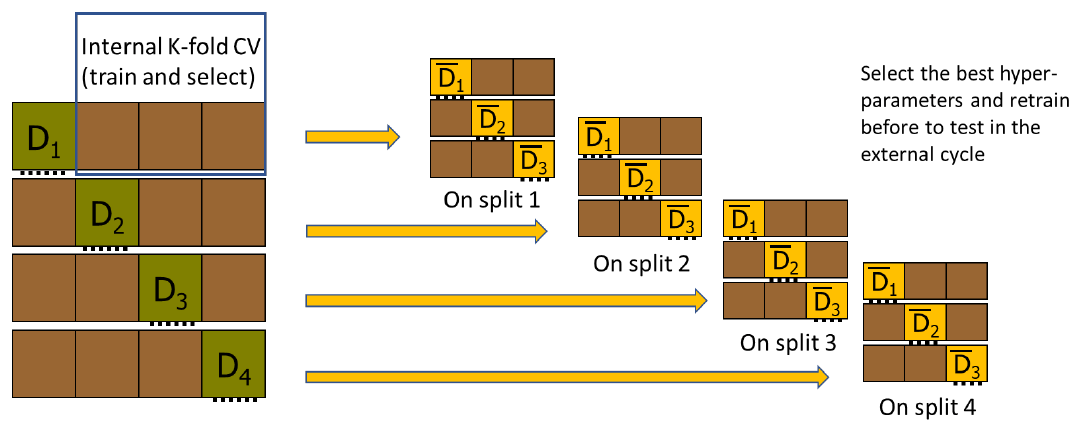
\includegraphics[width=0.89\linewidth,height=0.42\textheight,keepaspectratio]{images/10-val2_double-cv.png}
\caption{Double K-fold CV: in each outer split an inner CV selects the
hyperparameters.}
\end{figure}

Here too \textbf{no single final model is obtained}, because each outer
loop may choose different hyperparameters: one obtains an estimate of
the risk of the class of models/algorithm, together with its
\textbf{variance} (standard deviation over the folds). If a single
final model is needed, a \textbf{separate model selection} (hold-out or
K-fold CV) and a possible final retraining are carried out.

This does not violate the rules: the test error has already been
estimated and test results are never used for selection; the final
model will have an expected error within the estimated range. This is
why it is not simply true that ``the test always comes last'': here it
takes place \textbf{before} the last model selection (even if it may
seem counter-intuitive).

Double CV makes better use of \textbf{all} the data for training and
evaluation (both for selection and for assessment), at the price of a
high computational cost.

\begin{figure}[htbp]
\centering
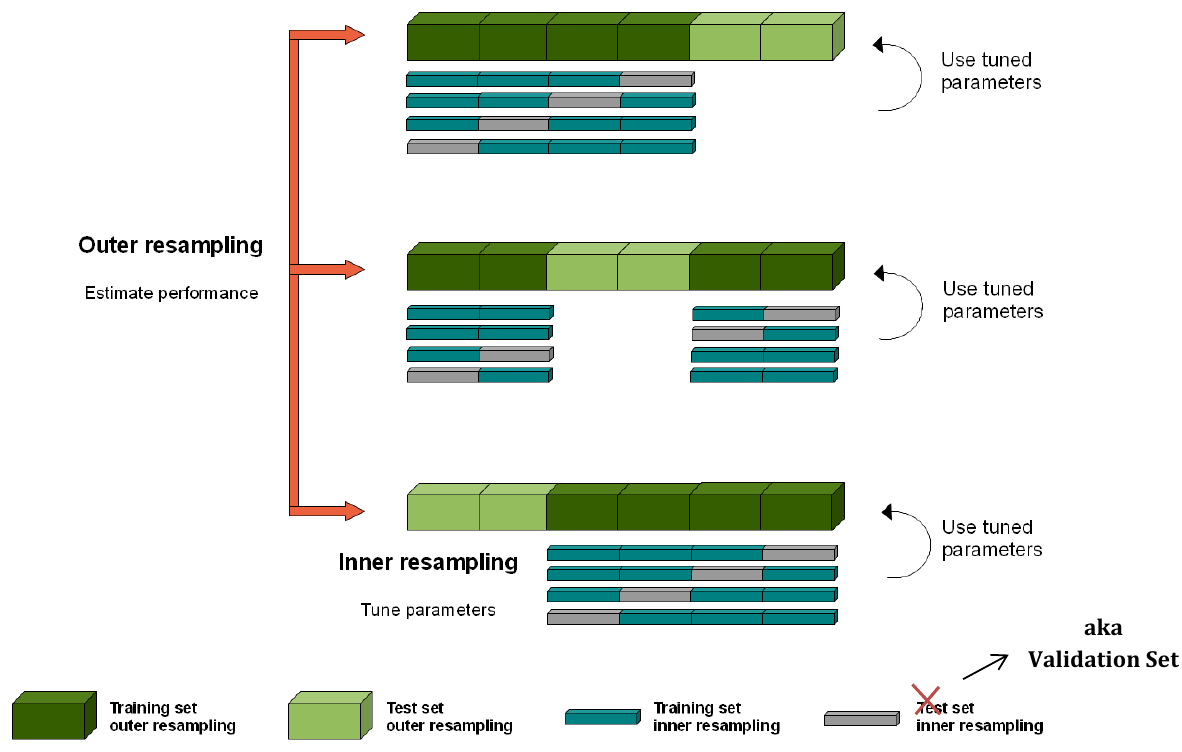
\includegraphics[width=0.80\linewidth,height=0.42\textheight,keepaspectratio]{images/10-val2_double-cv-2.png}
\caption{Another view of double CV: outer resampling to estimate the
performance, inner resampling to tune the parameters.}
\end{figure}

\begin{figure}[htbp]
\centering
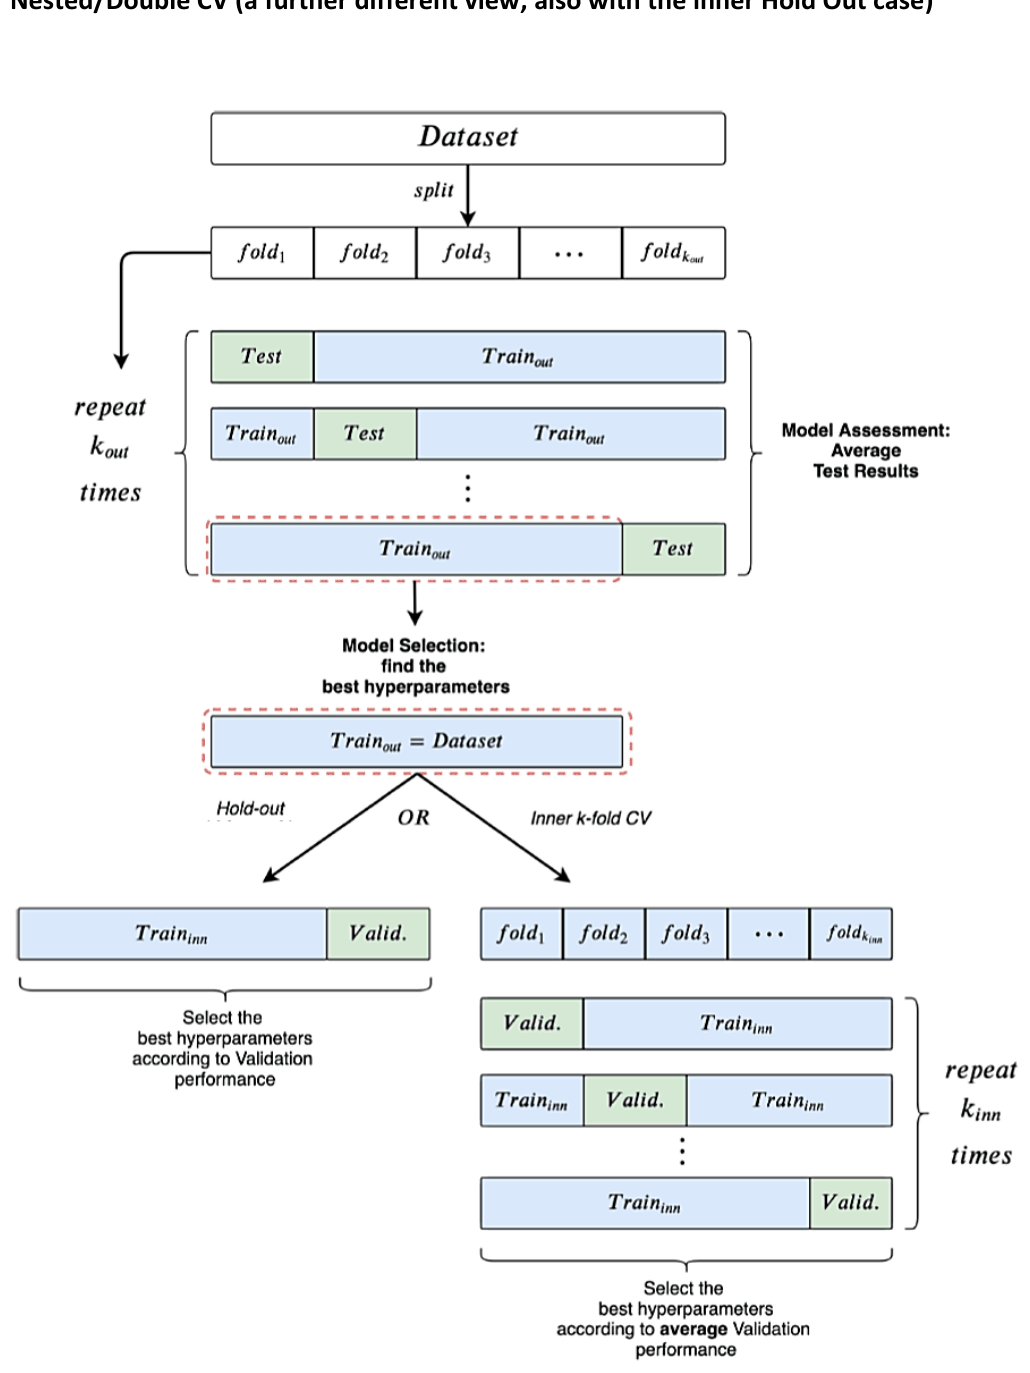
\includegraphics[width=0.63\linewidth,height=0.42\textheight,keepaspectratio]{images/10-val2_nested-cv.png}
\caption{Nested CV, also in the variant with internal hold-out.}
\end{figure}

\begin{boxabstract}{Summary}

First the goal is identified (best model, performance estimate, or
both), then the scheme is chosen. In all correct schemes: the
\textbf{test is separated before} any choice, the estimates on
\textbf{VL are not returned} as risk estimates, each CV iteration
\textbf{starts from scratch}. The most used combined schemes are
TR--VL--TS, CV+test and double CV.

\end{boxabstract}

\begin{boxquestion}{Possible exam questions}

\begin{itemize}
\tightlist
\item
  Write the model selection algorithm with K-fold CV.
\item
  Write the model assessment algorithm with K-fold CV.
\item
  Describe double (nested) CV. Does it return a model?
\item
  Relate errors (1) and (2) of the counterexample to the formal
  schemes.
\end{itemize}

\end{boxquestion}
